\chapter{Experimentos}
\label{cap:experimentos}

En este capítulo se muestra el resultado de una serie de experimentos que ayudan a validar y verificar el algoritmo implementado. Como se ha comentado anteriormente todas las pruebas se han hecho en un simulador en el entorno de la RoboCup SPL. \\

 A pesar de que muchas de las gráficas muestran únicamente la calidad de los objetos, en estos experimentos se hablará indistintamente de la calidad o de la incertidumbre de estos. Decir que disminuye la calidad o que aumenta la incertidumbre significa lo mismo, que la información del objeto es menos fiable.

\section{Seguimiento de un objeto}
\label{sec:seguimientoobjeto}

En este experimento se comparan los resultados obtenidos a partir de las observaciones obtenidas del detector y esas mismas observaciones procesadas mediante el algoritmo de seguimiento, figura \ref{fig:tracked_vs_raw_plot}. En este experimento se ha colocado una pelota a cierta distancia del robot y se ha teleoperado el robot de forma que vea la pelota en todo momento y se ha golpeado la pelota. Los datos que muestra la gráfica es la distancia a la que se encuentra la observación en cada instante de tiempo. La distancia está medida en milímetros. \\

\begin{figure} [h]
  \begin{center}
    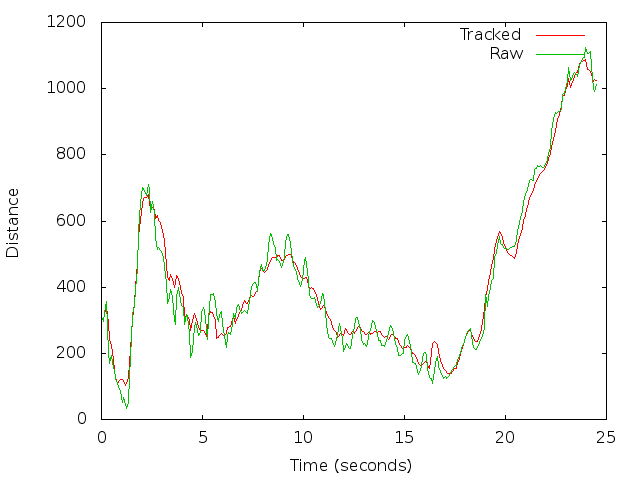
\includegraphics[width=13cm]{img/cap5/tracked_vs_raw_plot}
  \end{center}
  \caption{Distancia a la que se encuentra un objeto haciendo el seguimiento y tomando las medidas del detector directamente}
  \label{fig:tracked_vs_raw_plot}
\end{figure}

Las observaciones sin procesar son las de color verde. Se puede ver que la gráfica esta llena de picos y no es en absoluto estable. Ello se debe al ruido en las observaciones por causa del movimiento del robot e imprecisiones en la detección de la pelota. De color rojo se puede ver la observación procesada por el algoritmo de seguimiento. Se puede apreciar a simple vista como se mitigan las imprecisiones causadas por el ruido de las observaciones. Entre iteración e iteración existe una pequeña variación de la posición, pero bastante más reducida que las observaciones en crudo. \\

Uno de los efectos colaterales del procesado de las observaciones es la pérdida de reactividad frente a cambios en la posición del objeto. Se puede ver que los cambios en la observación procesada se producen más tarde en el tiempo que la observación en crudo. Este genera un pequeño desfase entre la posición real y la calculada por el algoritmo. Esta consecuencia es inevitable. Al modelar el objeto que se va a seguir, hay que elegir entre estabilidad y reactividad. Un objeto más estable se verá afectado en menor medida por el ruido de las observaciones, pero tardará más en reaccionar frente a un cambio en la posición del objeto. Si el objeto es más reactivo, ocurre los contrario. \\

\section{Descubrimiento de falsos positivos}
\label{sec:experimentofalsospositivos}

En este experimento se muestra como reacciona el algoritmo frente a los falsos positivos. La pelota se ha situado enfrente del robot. Éste hace barridos de un lado a otro con la cabeza de forma que a veces la ve y a veces no. En un momento dado, cuando el robot no está viendo la pelota, se quita de esa posición. \\

La gráfica de la figura \ref{fig:exp1} presenta la calidad del objeto a lo largo del tiempo. No se aprecia bien en la gráfica, pero en los primeros instantes de ejecución la calidad pasa de 0 a un valor cercano a 1 en cuanto el robot divisa la pelota. Aproximadamente a partir del segundo 5 el robot deja de ver la pelota y la calidad empieza a descender. La curva de descenso es bastante liviana porque no hay ruido añadido causado por el movimiento del robot. Ese descenso de la calidad se debe únicamente a los parámetros con los que se ha modelado la pelota. \\

\begin{figure} [h]
  \begin{center}
    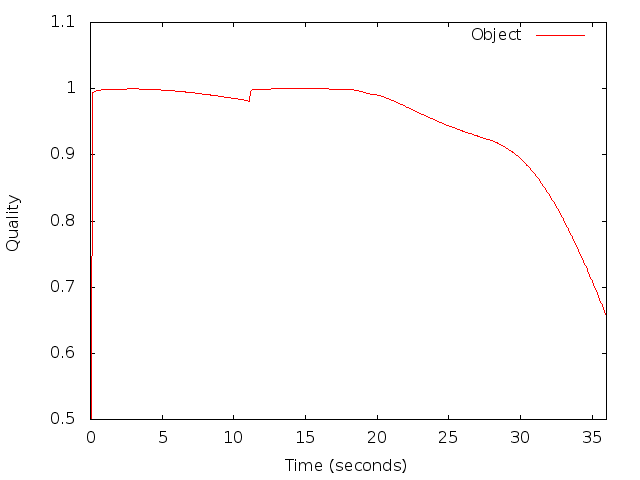
\includegraphics[width=13cm]{img/cap5/exp1.png}
  \end{center}
  \caption{Gráfico del experimento sobre los falsos positivos}
  \label{fig:exp1}
\end{figure}

Un poco después del segundo 10 se vuelve a localizar la pelota y la calidad vuelve a subir. Cuando se pierde otra vez de vista se puede apreciar una curva un poco distinta de la anterior. Ello se debe a que el objeto se encuentra en el límite de la imagen. Lidiar con estas situaciones es bastante difícil. El objeto se encuentra dentro del \textit{frustum} de la cámara, pero el detector no es capaz de reconocerlo. Esta situación hace que se considere el objeto como un falso positivo, lo que causa que la incertidumbre crezca más rápidamente. Esta situación prácticamente no afecta al rendimiento del algoritmo, pues se produce durante un espacio muy corto de tiempo. En cuanto el objeto se encuentra fuera del área de visualización de la cámara, éste deja de considerarse un falso positivo y vuelve a aumentar la incertidumbre al ritmo habitual. En la parte final de la gráfica se puede ver como cae en picado la calidad. Aquí es donde se ha retirado la pelota del sitio en el que estaba y el robot esta viendo que la pelota no se encuentra donde debería estar.\\

\section{Seguimiento de objetos con falsos positivos}
\label{sec:seguimientofalsospositivos}

En este experimento se demuestra el comportamiento del algoritmo cuando se está haciendo el seguimiento de un objeto y aparece un falso positivo. Éste hay que detectarlo y deshacerse de él cuanto antes para evitar equivocaciones. En esta prueba se ha colocado una pelota a cierta distancia del robot. Éste camina en línea recta hacia la pelota pudiendo verla en todo momento. En cierto momento aparece otra pelota, que simula ser un falso positivo, y desaparece. La gráfica \ref{fig:falsos_positivos} recoge la calidad de las dos pelotas a lo largo del tiempo. \\

\begin{figure} [h]
  \begin{center}
    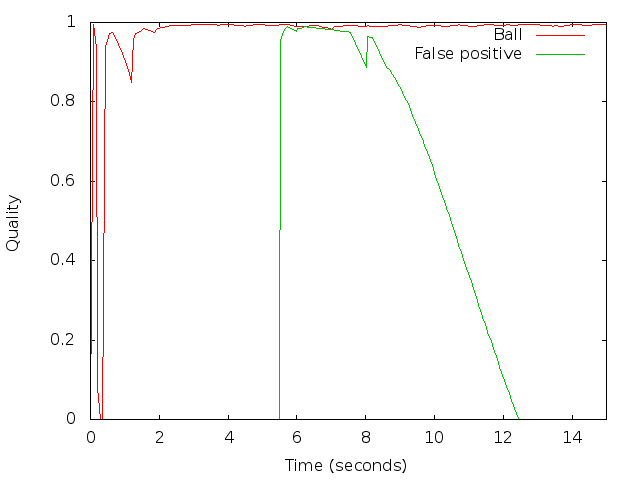
\includegraphics[width=13cm]{img/cap5/falsos_positivos}
  \end{center}
  \caption{Seguimiento de la pelota con un falso positivo}
  \label{fig:falsos_positivos}
\end{figure}

La línea de color rojo representa la calidad de la pelota. Al estar viéndola en todo momento, la calidad es muy alta. Tiene ligeras fluctuaciones que son causadas por el ruido de la observación y el desplazamiento del robot. La línea verde simula el falso positivo. Casi en el segundo 6 se detecta una posible pelota y se incorpora a la colección de pelotas. El falso positivo es detectado durante un breve período de tiempo y luego desaparece. Durante el tiempo que es detectado, no se llega a apreciar bien, pero la calidad del falso positivo es ligeramente menor que la calidad de la pelota real. Esto se debe a que la pelota real ha sido verificada durante muchas iteraciones anteriormente. \\

A partir del segundo 8 se pierde de vista por completo el falso positivo. En este momento, al encontrarse la última posición conocida del falso positivo dentro de la imagen, pero no encontrarse una observación en ese lugar, la calidad comienza a descender radicalmente. Este hace que se acabe por eliminar en poco más de 4 segundos. \\

Como se puede ver con este experimento, el algoritmo es robusto frente a falsos positivos. En el momento que se detecta que un filtro es un falso positivo o un objeto que ya no se encuentra en la imagen, se aumenta la incertidumbre mucho más rápido lo que hace que se acabe eliminando el filtro en un período corto de tiempo. \\

Existe un inconveniente muy difícil solucionar: las oclusiones. En caso de tener un objeto ocluido, éste se trataría como si fuese un falso positivo. Se tendría que utilizar algún método más elaborado para detectar si se puede tratar de una oclusión o no. \\

\section{Seguimiento de objetos complejos}
\label{sec:seguimientobjetoscomplejos}

Este experimento muestra el comportamiento del algoritmo cuando se hace el seguimiento de un objeto complejo, es decir, formado por varios objetos simples. El objeto en cuestión es la portería, formada por dos postes. El criterio para identificar una portería es simple: se comprueba la distancia entre los dos postes y las incertidumbres de estos. \\

Para este experimento se ha colocado un robot en el centro del campo mirando a una de las porterías. En el medio de la portería se ha colocado un poste adicional para que el robot vea tres postes y tenga que decidir cuáles son los que mejor identifican una portería. Durante todo el tiempo de la prueba se ha movido la cabeza de izquierda a derecha. La gráfica \ref{fig:exp2} muestra las calidades de cada uno de los postes. \\

\begin{figure} [h]
  \begin{center}
    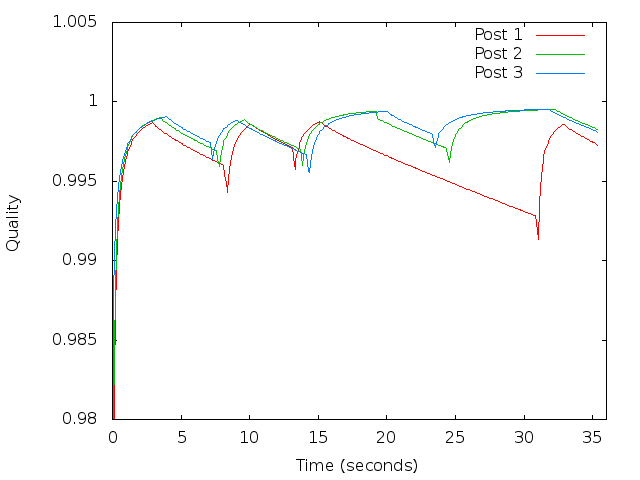
\includegraphics[width=15cm]{img/cap5/exp2.png}
  \end{center}
  \caption{Gráfico del experimento de seguimiento de objetos complejos}
  \label{fig:exp2}
\end{figure}

Las calidades de los postes aumentan y descienden de manera independiente al perderse de vista y volver a detectarse. A pesar de que las calidades varían, en todo momento el algoritmo detecta correctamente los postes de la portería, que son el 1 y el 3. Solamente en las primeras iteraciones, cuando la incertidumbre de los postes es bastante baja, hay algunos resultados erróneos. Se ha calculado que tiene aproximadamente un 99\% de fiabilidad. \\

Entre los segundos 25 y 30 se paró la cabeza del robot de forma que sólo viese uno de los postes de la portería y el poste falso. A pesar de disminuir la calidad del otro poste, la detección de la portería sigue siendo correcta. \\

Como ocurre en el primer experimento, se puede apreciar un comportamiento anómalo justo antes de volver a detectar los postes, una especie de ''V''. La calidad baja rápidamente y luego vuelve a subir. Al estar el poste en el límite de la imagen, la posición se encuentra dentro del frustum de la cámara, pero el detector no reconoce el objeto como un poste, por lo que se trata como si fuese un falso positivo. 

\section{Corrección de la velocidad de un objeto}
\label{sec:correcionvelocidadobjeto}

En este experimento se compara el resultado de actualizar la velocidad de un objeto cuando se interactúa con él y cuando no. La acción que se realiza es la de golpear la pelota. En este experimento se ha posicionado la pelota a una distancia cercana al robot y se ha activado el comportamiento \textit{Striker2}. Este comportamiento es el que utilizan los delanteros durante un partido. Realiza varias tareas complejas como buscar la pelota, aproximarse a ella y colocarse en posición para chutar entre otras. La figura \ref{fig:exp_kick_no_tracking} muestra el resultado del experimento, donde se puede ver el error en la posición de la pelota. \\

\begin{figure} [h]
  \begin{center}
    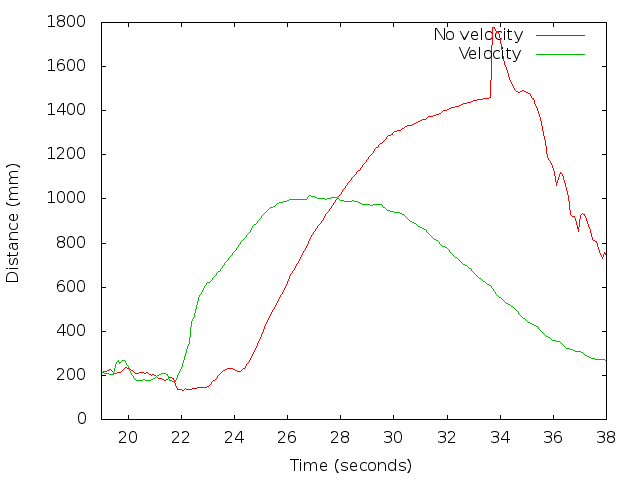
\includegraphics[width=15cm]{img/cap5/exp_kick_no_tracking}
  \end{center}
  \caption{Corrección de la velocidad de un objeto}
  \label{fig:exp_kick_no_tracking}
\end{figure}

La línea roja representa el experimento en el que no se ha actualizado la velocidad de la pelota cuando se la ha golpeado. En el momento en que se chuta, aproximadamente el segundo 24, se puede ver como empieza a aumentar en gran medida el error de la posición. Ello se debe a que la pelota se pierde de vista demasiado rápido y el robot \textit{cree} que sigue en la misma posición en la que estaba, justo enfrente. Únicamente tras un tiempo prudencial empieza a buscarla de nuevo, encontrándola  otra vez en el segundo 34. Durante esos 10 segundos el robot no sólo tenía una posición errónea de la pelota sino que se quedaba sin hacer nada, esperando encontrar la pelota en una posición que ya no está. \\

La línea verde representa el experimento en el que sí se actualizó la velocidad de la pelota. En este caso es en el segundo 22 cuando se golpea la pelota, y entonces el error de la posición también aumenta igual que antes, pero lo hace con antelación. Esto se debe a una desincronización entre el momento del golpeo y la actualización de la velocidad. Lo ideal sería que se actualizase la velocidad en el momento exacto del golpeo, pero el sistema robótico utilizado no permite detectar tal situación, por lo que se actualiza la velocidad un poco antes del golpeo real de la pelota, justo en el momento en el que se decide dar una patada a la pelota. \\

Al actualizar la velocidad de la pelota, ésta comienza a alejarse del robot. El módulo de atención visual que utiliza el comportamiento \textit{Striker2} se ve obligado a levantar la cabeza del suelo para mirar las nuevas posiciones de la pelota y, de ese modo, es capaz de ver la pelota real alejándose del robot. Por esto se detecta mucho antes la pelota y se pueden tomar nuevas decisiones mucho más rápido. El algoritmo predice la nuevas posiciones provocando un mejor comportamiento del sistema. Si antes fueron necesarios 10 segundos para localizar de nuevo la pelota, al actualizar la velocidad de la pelota en poco más de 4 segundos el robot ha localizado de nuevo la pelota y puede seguir jugando. \\

\section{Tiempos de ejecución}
\label{sec:tiemposejecucion}

Por último se mide el tiempo de ejecución del algoritmo cuando se estima la posición de varios objetos, figura \ref{fig:10_balls}. En este experimento se han introducido uno a uno objetos en el campo de visión del robot hasta un total de 10. Al cabo de un corto período de tiempo, de la misma manera, se han retirado uno a uno los objetos. \\

El tiempo de ejecución aumenta según aparecen objetos en el campo de visión del robot. Se puede ver que, para 10 instancias, el algoritmo se ejecuta en menos de 1 milisegundo. Cuando se empiezan a retirar los objetos el tiempo vuelve a decrecer al mismo ritmo que subía al principio del experimento. Estos tiempos son suficientes para ejecutar el algoritmo en tiempo real. \\

Los resultados obtenidos son satisfactorios. Al tener más objetos en el campo de visión, el algoritmo tarda más en ejecutarse, pero el tiempo de ejecución aumenta, no de manera lineal, pero a un ritmo sostenible. \\

\begin{figure} [h]
  \begin{center}
    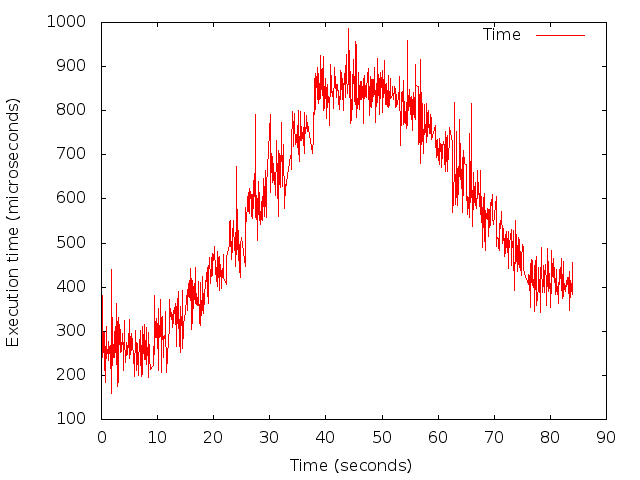
\includegraphics[width=13cm]{img/cap5/10_balls}
  \end{center}
  \caption{Gráfico con tiempos de ejecución}
  \label{fig:10_balls}
\end{figure}
